%EXP

\subsection{Experimental Setup}

Each bag of reads was assembled with SOAPdenovo2, which took 7-30 minutes per file, depending on the file size. The assembly of the patient files is embarrassingly parallel, so the assembly of each file could be done at the same time. Combining the files into one file took 2 minutes and 35 seconds. Assembly was used for all of the classification methods tested, because the combining of individual reads and reduction in total data size made classification feasible.

\subsection{Methods Tested}

This section provides an overview of the different methods that we compared our pipeline to. Our pipeline uses clustering, whereas the other methods do not. Instead, those methods directly compare individual reads instead of clusters. In order to do this, sequence reads were represented as counts of k-mers. %k-mers are nucleotide strings of length k. Since there are four possible nucleotides, the number of possible k-mers is \(4^k\). 
%For instance, if k=3, there are \(4^3\) = 64 possible k-mers, which are AAA, AAC, AAG, AAT, ACA, ACC, ..., TTT. 
%For a string "ATACGATA", the count for the k-mers is 2 for ATA, 1 for TAC, ACG, CGA, and GAT, and 0 for everything else. 
We wrote a script to represent the reads/contigs as vectors representing the k-mer counts in the string, and these feature 
vectors were used by the other methods. We tested possible k values 
from 1 to 6; since the number of possible k-mers is 
exponential in k, higher values for k quickly become impractical in both run time and memory usage. From experimental validation, we found a k-mer value of 3 to be the most effective. Converting the reads from their string form to k-mer vectors with k=3 took 24 hours, 8 minutes, 49 seconds.

%%%%%%%%%%%%%%%%%%%%%%%%%%%%%%%%

\subsubsection{CAMIL - Our Pipeline}

We implemented two different versions of the pipeline in Python: one that uses D-BoW feature extraction, and one that uses H-BoW feature extraction. These results are denoted as ``CAMIL D-BoW" and ``CAMIL H-BoW", respectively, in the results tables and graphs. Clustering for the pipeline with UCLUST took 14 hours, 7 minutes, 44 seconds. All 367 patients were clustered together in order to keep the features consistent.

\subsubsection{MISVM and sbMIL}

MISVM \cite{andrews02} and sbMIL \cite{bunescu07} are two of the classic Multiple Instance Learning algorithms that fall into what Amores calls the ``Instance Space" (IS) methods, in that they only use ``local" information based on comparisons between individual instances and treat bag labels as aggregations of instance labels \cite{amores13}. Additionally, both of these methods follow the standard MIL assumption that bags with negative labels contain only negative instances, whereas positive bags contain one or more positive instances \cite{amores13}. sbMIL specifically assumes that positive bags contain few positive instances \cite{bunescu07}. We include these algorithms as an example of many of the early MIL algorithms, which usually fell into the IS paradigm and used the standard MIL assumption. For the implementation of these methods, we used an open-source Python implementation by Doran \cite{doran14}, which is available on GitHub\footnote{https://github.com/garydoranjr/misvm}.

\subsubsection{GICF}

The Group-Instance Cost Function (GICF) is a method proposed by Kotzias et al. that learns instance labels in addition to group labels \cite{kotzias15}. The cost function uses a kernel that measures similarity between instances and a penalty on the difference between instance labels to generate instance labels \cite{kotzias15}. It then sets the group label to be the average instance label of all instances in that group, using a penalty on the difference between the predicted group label and the actual group label \cite{kotzias15}. Ideally, this would cause instances that are similar to each other to have similar predicted labels, and predicted group labels to correspond closely to reality. Unlike MISVM and sbMIL, GICF explicitly does not hold the standard MIL assumption, instead favoring the collective assumption. However, because this method compares only individual instances and not entire bags, and treats bag labels simply as aggregations of instance labels, GICF is still an Instance Space method. GICF is a generalized cost function, but the authors also use a specific version of it in their paper with squared loss for bag and instance level errors and logistic regression for classification \cite{kotzias15}; this is the specific version that we implemented in Python. Like Kotzias et al. \cite{kotzias15}, we used mini-batch stochastic gradient descent with momentum to train the classifier and linear grid search to pick the parameters.

\subsubsection{Original MGWAS Paper}

The methods used by Qin et al. \cite{qin041012} are neither MIL-based, nor are they entirely de novo apart from patient labels. The authors first performed de novo assembly with SOAPdenovo2 \cite{luo12} and then used a tool called MetaGeneMark \cite{zhu10, besemer99} for de novo prediction of genes from the assembled contigs \cite{qin041012}. They then combined these genes with an existing gene catalog, MetaHIT \cite{qin030410}, and carried out taxonomic assignment and functional annotation of the genes using the KEGG \cite{kanehisa00} and eggNOG \cite{powell12} databases, as well as 2,890 other reference genomes \cite{qin041012}. The authors defined gene markers by mapping the sequence reads from the MGWAS dataset to the updated gene catalog. They identified the 50 most important gene markers with the minimum redundancy - maximum relevance (mRMR) \cite{peng05} method, using the ``sideChannelAttack" R package and then used these 50 gene markers for SVM classification of T2D phenotype, using the ``e1071" R package for the SVM \cite{qin041012}. Thus, the method in the original paper first applies de novo assembly and gene prediction methods, but then uses a number of references to identify the gene markers to be used in classification. From their results, the authors generated an Area Under Curve - Receiver Operating Characteristic (AUC-ROC) graph. The authors did not provide a learned decision boundary in their supplementary tables, only the predicted values for each patient, so we manually computed the accuracy and F1 score with an optimally-chosen decision boundary. 

%%%%%%%%%%%%%%%%%%%%%%%%%%%%%%%%


\subsection{Results For Bag/Patient Labels}

\begin{table}[h]
\begin{center} 
%\hfill
\caption{Performance with even train/test split.} 
\label{tab:even-comp}
\begin{tabular}{|c|ccc|}\hline
Method & Accuracy & F1-Score & AUC-ROC\\\hline
MISVM & --- & --- & ---\\\hline
sbMIL & --- & --- & ---\\\hline
GICF & 63.04 & 68.33 & 66.19\\\hline %59.24,63.05,66.19
CAMIL D-BoW & 86.34 & 87.18 & 95.93\\\hline
CAMIL H-BoW & \bf{90.71} & \bf{89.70} & \bf{97.63}\\\hline
\end{tabular}
\end{center}
\end{table}

\begin{table}[h]
\begin{center}
\caption{Classification time and memory usage with even train/test split.} 
\label{tab:time-comp}
\begin{tabular}{|c|cc|}\hline
Method & Classification Time & Memory Usage\\\hline
MISVM & --- & Memory Error\\\hline
sbMIL & --- & Memory Error\\\hline
GICF & 8 hours, 44 mins, 27 secs & 2.646 GB\\\hline
CAMIL D-BoW & \bf{6 minutes, 58 seconds} & \bf{545.293 MB}\\\hline
CAMIL H-BoW & 7 minutes, 56 seconds & 546.297 MB\\\hline
\end{tabular}
\end{center}
\end{table}

In the original MGWAS paper, the authors use 344 patients as a training set and 23 as a test set. However, when comparing to other MIL algorithms, we wished to have a more balanced training vs. test set split. We put 184 patients in the training set and 183 in the test set. Since this used a different training set than the one in the MGWAS paper, we do not compare our results to theirs here. Table \ref{tab:even-comp} shows the comparison of results between CAMIL, GICF, MISVM, and sbMIL, while Table \ref{tab:time-comp} compares the classification time and memory usage. CAMIL methods significantly outperform GICF, with the H-BoW variant of CAMIL slightly outperforming the D-BoW variant. CAMIL took significantly less time than GICF for two main reasons: (i) GICF requires representing each read as an array of length 64 (for k-mer length 3), while CAMIL reduces the data size with clustering and feature extraction; (ii) GICF requires expensive pairwise comparisons between each pair of instances in a mini-batch. MISVM and sbMIL require computing a kernel matrix of size N*N, where N = the number of instances. Since this dataset involved millions of instances, these methods crashed with memory errors. This is why they are shown as ``---" in the results tables.

\begin{table}[h]
\begin{center}
\caption{Performance on subset of instances with even train/test split.}
\label{tab:subset-comp}
\begin{tabular}{|c|ccc|}\hline
Method & Accuracy & F1-Score & AUC-ROC\\\hline
MISVM & 50.8 & --- & 48.47\\\hline
sbMIL & 50.8 & --- & 48.47\\\hline
GICF & 64.67 & 66.95 & 65.56\\\hline
CAMIL D-BoW & \bf{84.15} & \bf{85.13} & \bf{90.86}\\\hline
CAMIL H-BoW & 74.32 & 68.46 & 83.49\\\hline
\end{tabular}
\end{center}
\end{table}

We wanted to compare MISVM and sbMIL to GICF and CAMIL, so we used a subset of the instances for each patient so that MISVM and sbMIL would not crash. They could only be run on 0.1\% of the reads for each patient, and even then took over 32.5 GB of memory. The results are shown in Table \ref{tab:subset-comp}. MISVM and sbMIL also only achieved 50.8\% accuracy, only slightly better than a random guess. The F1 score could not be computed because there were no True Positives or False Positives. GICF and CAMIL, while experiencing a performance drop due to the massive information loss, still performed much better, with the CAMIL methods outperforming GICF again. CAMIL D-BoW outperformed CAMIL H-BoW this time, because the distance calculations are less affected by having fewer reads than the histogram method.

MISVM and sbMIL performed the worst overall. This makes sense, as they make the standard MIL assumption, which doesn't make sense in the context of phenotype prediction, in which even healthy patients can host a small number of pathogens. Additionally, they are instance space methods that do not leverage bag-level information. The performance of these two methods serves to illustrate why many of the classic MIL algorithms with standard assumptions will not be effective in this domain. GICF performs better than MISVM and sbMIL, which makes sense given the fact that it follows the collective assumption. It also has the benefit of calculating instance labels, which we explore further in the next section. However, GICF is still an instance space method, so it makes sense that CAMIL outperformed it.

\begin{table}[h]
\begin{center}
\caption{Performance with 23 patient test set.} 
\label{tab:test-comp}
\begin{tabular}{|c|ccc|}\hline
Method & Accuracy & F1-Score & AUC-ROC\\\hline
mRMR + SVM & 80.00 & 81.20 & 82.30\\\hline 
CAMIL D-BoW & 91.62 & 91.89 & \bf{98.03}\\\hline
CAMIL H-BoW & \bf{95.59} & \bf{95.20} & 97.93\\\hline
\end{tabular}
\end{center}
\end{table}

Table \ref{tab:test-comp} compares CAMIL to the method used by Qin et al., mRMR + SVM. We initially tested CAMIL on the same 23 patient test set that Qin et al. used, for which CAMIL H-BoW had 100\% accuracy and AUC, while mRMR + SVM had 0.81 AUC as reported by Qin et al. \cite{qin041012}. We know CAMIL is not 100\% accurate, so we validated it by averaging the results of 10 independent trials in which we selected 23 patients randomly out of the 367 to serve as the test set, with the other 344 of the training set. Table \ref{tab:test-comp} shows that CAMIL significantly outperformed mRMR + SVM on these trials, with the H-BoW variant of CAMIL slightly outperforming the D-BoW variant.

Unlike the other MIL methods, Qin et al. use reference genomes to inform their classifier, so it makes sense that their method performs better than the MIL methods that only use de novo techniques. However, CAMIL still significantly outperformed the results reported in the MGWAS paper. We believe that the primary reason for this is that Qin et al. relied on alignments of sequences to reference genomes and attempted to select the 50 most significant genes for the phenotype before building the classifier. There are two primary problems with this approach: (i) many microbes found in the gut do not exist in reference databases and would thus be unusable for their classifier, and (ii) by only using 50 genes to inform the classifier, a lot of potentially valuable data is left out. CAMIL avoids these issues by using as much data as can be assembled and not relying on reference databases. The tradeoff is that we don't know exactly what genes are being used by the classifier to form the decision boundary. We also believe that the clustering process of putting similar contigs into groups forms useful features for the classifier.

\subsection{Cluster-level ``Labels"}

\begin{figure}[h]
\centering
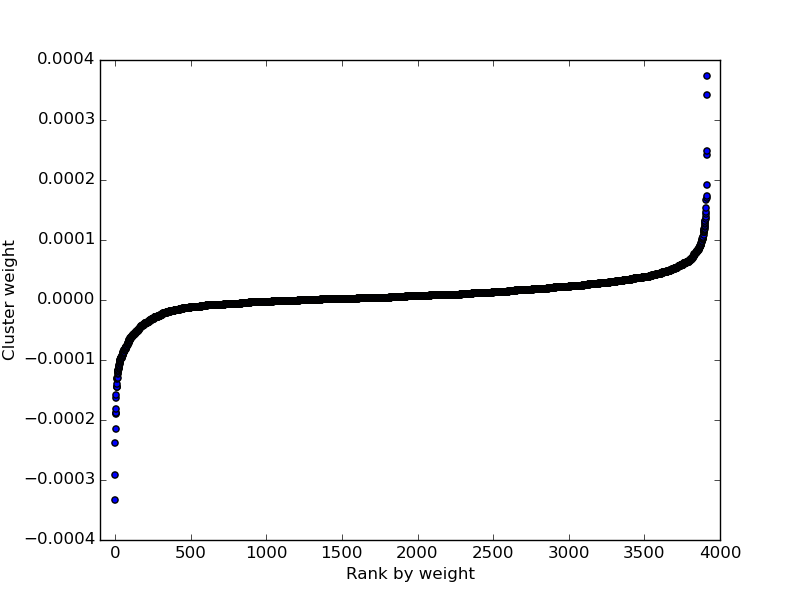
\includegraphics[scale=0.4]{./instance-scatter.png}
\caption{This diagram illustrates the distribution of the instance weights assigned by CAMIL H-BoW. The Y-Axis shows the weights, while the X-Axis shows the ranking of the clusters by weight. Clearly, there are a relatively small number of clusters that have disproportionately large weights or small weights, while the vast majority of the 3918 clusters have weights close to 0.} \label{instance-scatter}
\end{figure}

In the original MGWAS paper, the authors identify 50 important gene markers with mRMR that are used for their classifier. Conversely, CAMIL uses all of the data to train and test the classifier, resulting in 3918 clusters, and subsequently identifies significant clusters based on the classification results. Figure \ref{instance-scatter} is a visual display of the cluster weights determined by CAMIL, using the 344 patient training set and 23 patient test set. Clearly, there are a few clusters with disproportionately high or low weights, while most clusters have weights near 0. Concretely, the lowest cluster weight is -0.000333, the highest is 0.000374, the mean is 0.000008, and the median is 0.000006. Intuitively, this appears to make sense, as there should be a relatively small number of key clusters whose presence is actually indicative of type 2 diabetes, while most other clusters are not particularly relevant in this case and whose weights are just noise. Thus, the weights obtained by this method appear to be plausible. In contrast, the labels obtained by GICF were barely differentiated from each other at all.
